%\svnInfo $Id$
%\svnKeyword $HeadURL$

%\documentclass{article}
%\usepackage{epsfig}
%\begin{document}

\subsubsection{Visualization and Computer Graphics}
\index{Linsen, Lars}

\paragraph{Research Team}
Lars Linsen (Professor),
Sherin Al-Shbat (PhD Student),
Tetyana Ivanovska (PhD Student),
Tran Van Long (PhD Student),
Paul Rosenthal (PhD Student)\\

The Visualization and Computer Graphics Laboratory (VGCL) led by Prof.~Lars Linsen is
mainly concerned with topics from scientific and information visualization plus some
selected topics from computer graphics and geometric modeling.

Visualization is an inherently interdisciplinary field with application in many different
areas.  Scientific visualization deals with the visualization of data with spatial
interpretation such as computer-generated data from numerical simulations (physics,
chemistry) or measured data using scanning or sensoring techniques (medicine, life
sciences, geosciences).  The group's efforts are to generate visualization methods that
can handle large data sets efficiently, filter distinct features automatically or
interactively, and display the relevant information in a comprehensive and intuitive
fashion.  The research focuses on segmentation and isosurface extraction, hierarchical
methods, multi-variate data visualization, flow and tensor field visualization, and user
interaction.

Information visualization deals with the visualization of abstract data with no spatial
interpretation such as graph- or network-based data (life sciences, social sciences) or
multi-dimensional data (databases, ecomomics).  The group's efforts focus on interactive
exploration and analysis tools for such abstract data.

In the areas of computer graphics and geometric modeling the group's interest lies in
point-based methods, multi-resolution surface representation, and curves on surfaces.


\paragraph{Highlights} \ \\

{\em Direct Isosurface Extraction from Scattered Volume Data.}
Isosurface extraction is a standard visualization method for scalar volume data and has
been subject to research for decades.  Nevertheless, no isosurface extraction method
existed that directly extracts surfaces from scattered volume data without 3D mesh
generation or reconstruction over a structured grid. We have developed a method based on
spatial domain partitioning using a $k$d-tree and an indexing scheme for efficient
neighbor search. Our approach consists of a geometry extraction and a rendering step. The
geometry extraction step computes points on the isosurface by linearly interpolating
between neighboring pairs of samples. The neighbor information is retrieved by
partitioning the 3D domain into cells using a $k$d-tree. The cells are merely described by
their index and bitwise index operations allow for a fast determination of potential
neighbors. The final rendering step uses point-based rendering techniques.

\begin{figure}[ht]
  \begin{center}
    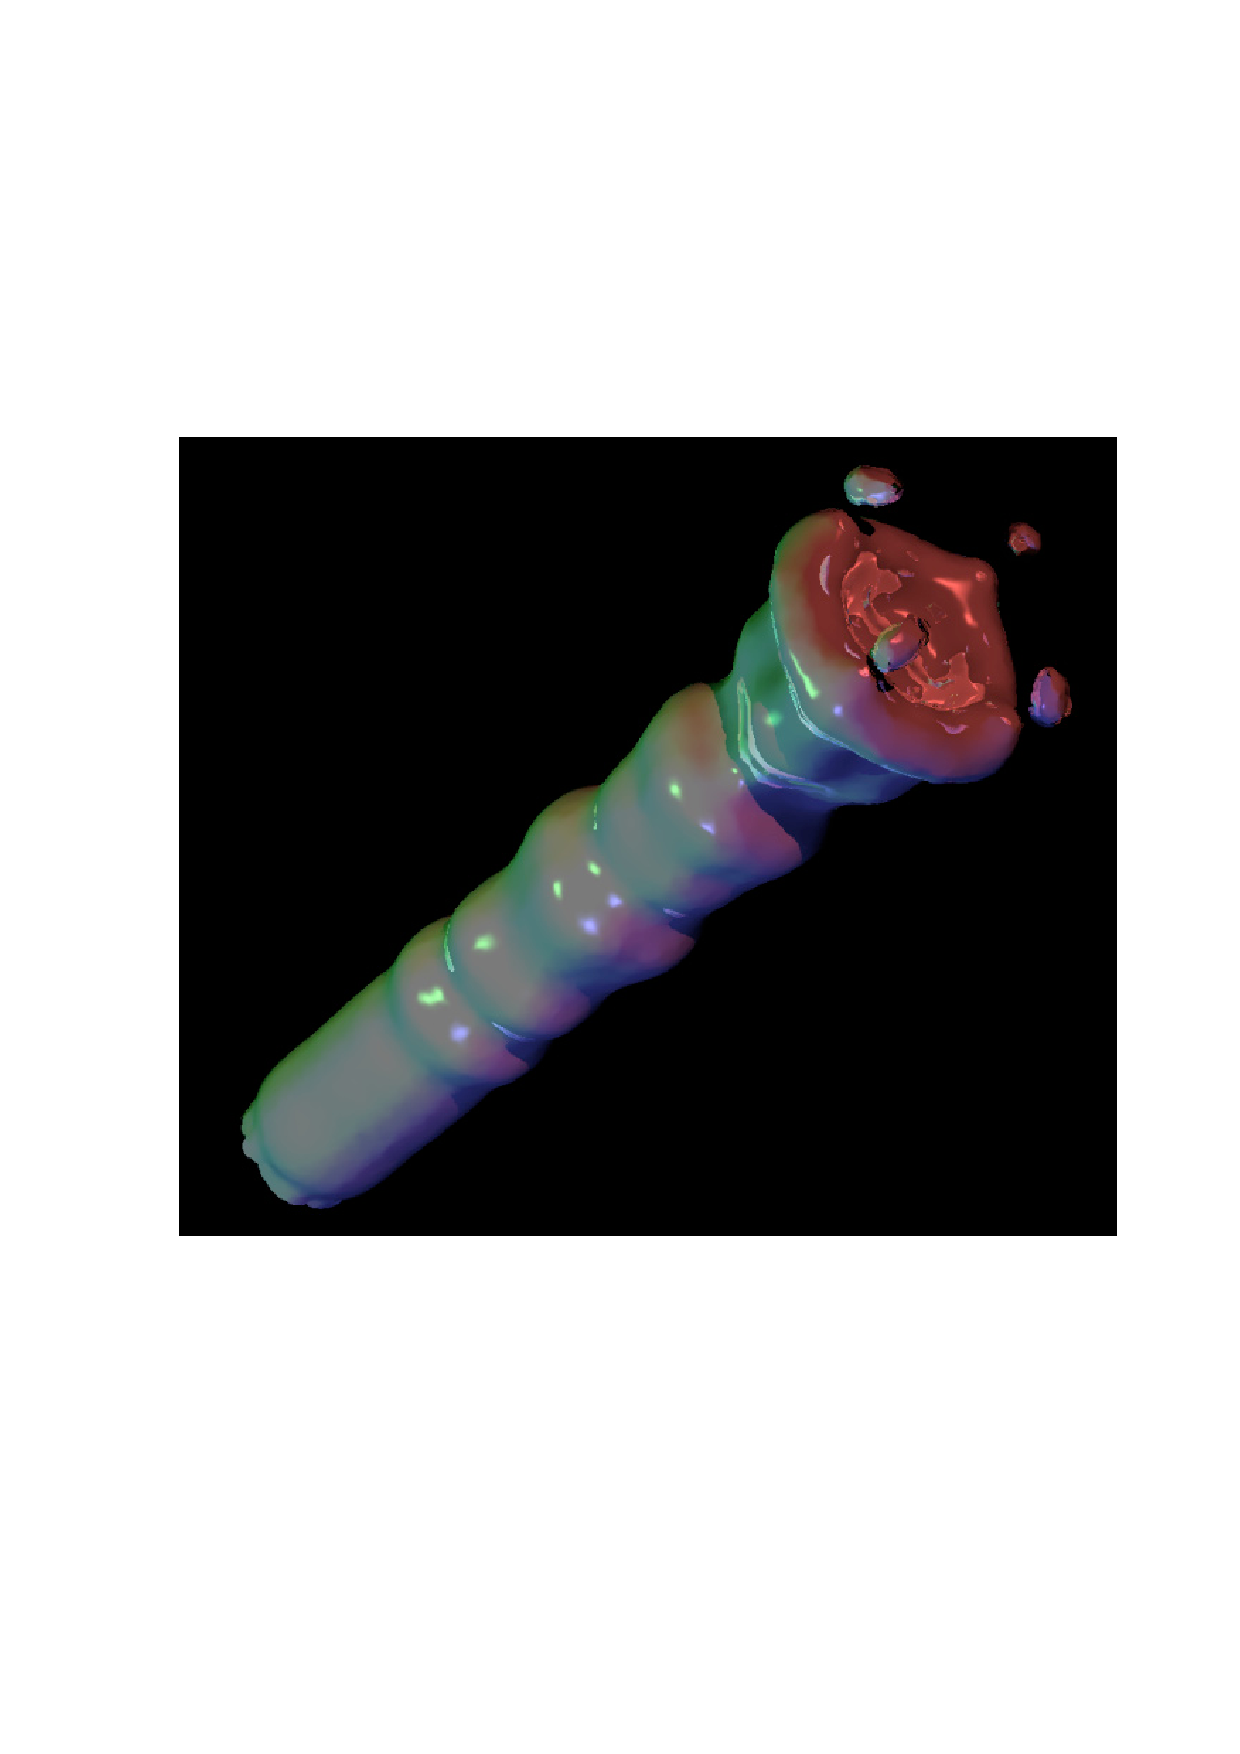
\includegraphics[width=\hsize]{Linsen_2006_Fig1.pdf}
    \caption{Point-based ray tracing of isosurface directly extracted from a scattered
      volume data. The scattered data set is a uniform random sampling of simulation data
      of fuel injection into a combustion chamber.}
    % \caption{Point-based ray tracing of isosurface directly extracted from a scattered
    %   volume data. The scattered data set is a uniform random sampling of simulation
    %   data of fuel injection into a combustion chamber.}
    % \label{fig:profxxx}
   \end{center}
\end{figure}

\noindent
{\em Using Ray Intersection for Dual Isosurfacing.}
Isosurface extraction using dual contouring approaches have been developed to generate a
surface that is dual in terms of the underlying extraction procedure used when compared to
the standard Marching Cubes (MC) method. These approaches address some shortcomings of the
MC methods including feature-detection within a cell and better triangles. We have
developed a simple method based on the MC method and the ray intersection technique to
compute isosurface points in the cell interior. One of the advantages of our method is
that it does not require Hermite data, i.e., the discrete scalar values at vertices
suffice. We compute ray intersections to determine isosurface points in the interior of
each cell, and then performed a complete analysis of all possible configurations to
generate a look-up table for all configurations.  We use a look-up table to optimize the
ray intersection method to obtain minimum number of points necessarily sufficient for
defining topologically correct isosurfaces in all possible configurations.

\noindent
{\em Structure-accentuating Dense Flow Visualization.}
Vector field visualization approaches can broadly be categorized into approaches that
directly visualize local or integrated flow and approaches that analyze the topological
structure and visualize extracted features. Our goal was to come up with a method that
falls into the first category, yet reveals structural information. We have developed a
dense flow visualization method that shows the overall flow behavior while accentuating
structural information without performing a topological analysis. A flow integration step
generates a density field by tracing particles under the influence of the underlying
vector field. The resulting density is high in attracting regions and low in repelling
regions. Density is measured by the number of particles per region accumulated over
time. The density fields for forward and backward propagation are explored using
texture-based rendering techniques.  We obtained dense flow visualizations that display
the overall flow behavior, emphasize critical and separating regions, and indicate flow
direction in the neighborhood of these regions.

\begin{figure}[ht]
  \begin{center}
     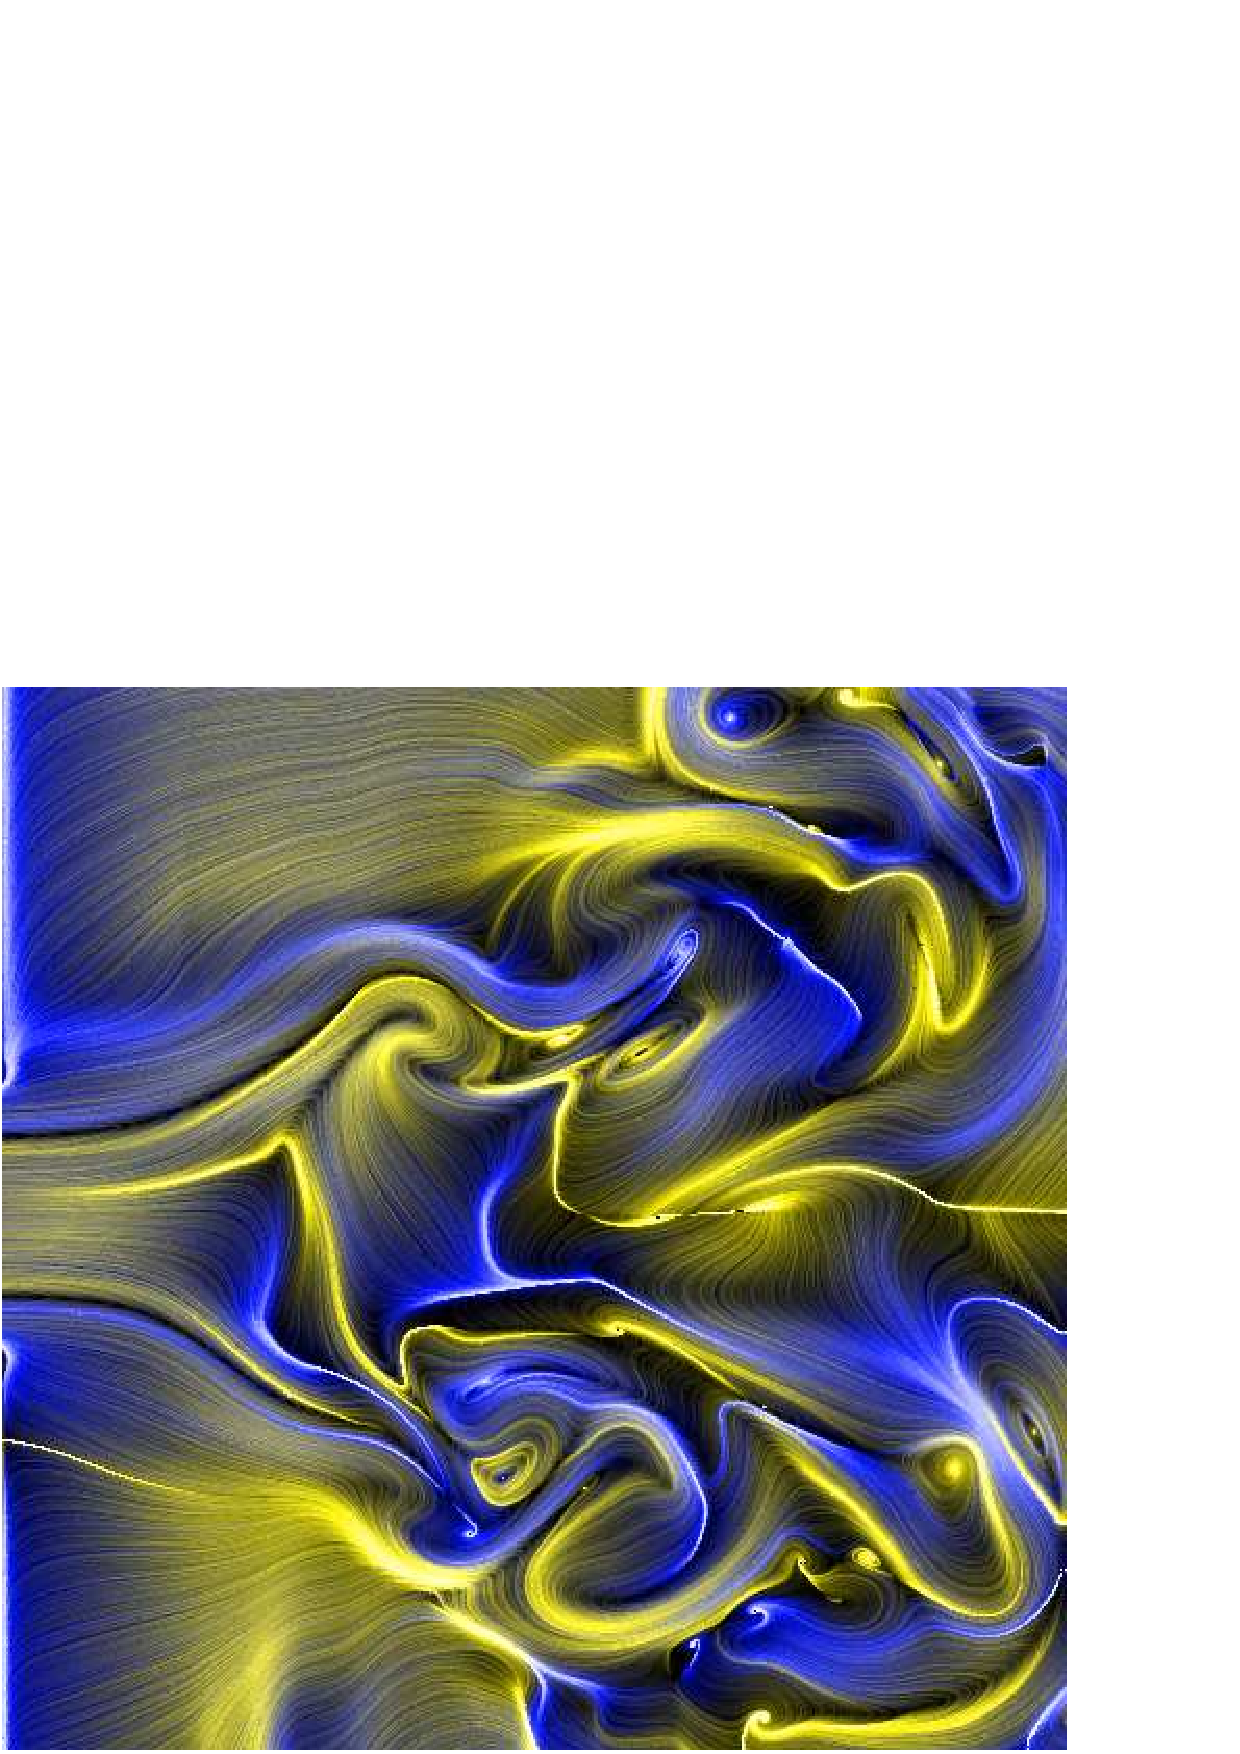
\includegraphics[width=\hsize]{Linsen_2006_Fig2.pdf}
    \caption{Structure-accentuating dense flow visualization applied to 2D simulation of
      a swirling jet.}
    %\caption{Structure-accentuating dense flow visualization applied to 2D simulation of a swirling jet.}
     % \label{fig:profxxx}
   \end{center}
\end{figure}

\noindent
{\em Visual Analysis of Gel-free Proteome Data.}
We developed a visual exploration system supporting protein analysis when using gel-free
data acquisition methods. The data to be analyzed is obtained by coupling liquid
chromatography (LC) with mass spectrometry (MS). LC-MS data has the properties of being
non-equidistantly distributed in the time dimension (measured by LC) and being scattered
in the mass-to-charge ratio dimension (measured by MS).  A hierarchical data
representation and visualization method is used for large LC-MS data. Based on this
visualization we have developed a tool that supports various data analysis steps like
deisotoping, landmark-based registration, and differential protein expression
analysis. Our visual tool provides a global understanding of the data, intuitive detection
and classification of experimental errors, and extensions to LC-MS/MS, LC/LC-MS, and
LC/LC-MS/MS data analysis.


\paragraph{Organization}
% list the (research) events you have organized, if any,

\begin{enumerate}
\item International conference on {\em Visualization in Medicine and Life Sciences (VMLS
    06)} held July 19--21, 2006, at Binz, R{\"u}gen, Germany
  (http://www.lars-linsen.de/vmls).  Organizers: Lars Linsen, Hans Hagen (University of
  Kaiserslautern), and Bernd Hamann (University of california, Davis).
\end{enumerate}

\paragraph{Collaborations}
\begin{enumerate}
\item {\sl Institut f{\"u}r Mathematik und Informatik, Ernst-Moritz-Arndt-Universit{\"a}t Greifswald, Germany}.\\
  Prof.~Georg F{\"u}llen, Julia L{\"o}cherbach, Steffen Rudnick.\\
  (1) Visualization of protein-protein interaction. \\
  (2) Visualization of gel-free proteomics data.\\
  (3) Simulation and animation of urban tree growth.
\item {\sl Institut f\"ur Mikrobiologie, Ernst-Moritz-Arndt-Universit\"at
    Greifswald, Germany}. \\
  Prof.~Michael Hecker, Dr.~J{\"o}rg Bernhardt, Dr.~D{\"o}rte Becher.\\
  Visualization of gel-free proteomics data.
\item {\sl Decodon GmbH, Greifswald, Germany}. \\
  Dr.~Matthias Berth, Dr.~J{\"o}rg Bernhardt.\\
  Visualization of gel-free proteomics data.
\item {\sl Institut f\"ur Diagnostische Radiologie und Neuroradiologie,
    Ernst-Moritz-Arndt-Universit\"at
    Greifswald, Germany}. \\
  Prof.~Norbert Hosten, Dr.~S{\"o}nke Langner, Martin Domin. \\
  Glyph- and tracking-based visualization of diffusion MRT data.
\item {\sl Poliklinik f\"ur zahn\"arztliche Prothetik und Werkstoffkunde,
    Ernst-Moritz-Arndt-Universit\"at
    Greifswald, Germany}. \\
  Prof.~Bernd Korda{\ss}.\\
  Virtual placement and interactive optimization for functional occlusion in
  prosthodontics.
\item {\sl Institut f\"ur Psychologie, Ernst-Moritz-Arndt-Universit\"at
    Greifswald, Germany}. \\
  Prof.~Klaus Landwehr.\\
  An interactive system for the generation of symmetric images with respct to symmetry
  groups.
\item {\sl Fraunhofer-Institut f\"ur Produktionstechnologie, Aachen, Germany}. \\
  Prof.~Christian Brecher, Prof.~Fritz Klocke, Lothar Glasmacher, Dr.~Olaf Dambon, Richard Zunke, Timo Wenzel.\\
  MoldFinish: Intelligent polishing system for automated finishing in tool and mold
  making.
  % (1) MoldFinish: Intelligents Poliersystem zur Automatisierung und Endbearbeitung im Werkzeug- und Formenbau.\\
  % (2) IProM: Multi-senorielle Messtechnik in Produktionsmaschinen
\item {\sl Institute for Data Analysis and Visualization (IDAV), University of California,
    Davis, U.S.A.} \\
  Prof.~Bernd Hamann, Prof.~Kenneth I.~Joy, Prof.~Nina Amenta, Prof.~John D.~Owens, Prof.~Oliver G.~Staadt, Dr.~Oliver Kreylos, Dr.~David F.~Wiley, Sung Park, Jaya Sreevalsan-Nair. \\
  (1) New approaches in flow visualization.\\
  (2) Exact dual isosurface extraction.\\
  (3) Interactive visual exploration of Northern California's water monitoring network.\\
  (4) Surface-based brain morphing.
\item {\sl Zuse Institut Berlin, Germany.}\\
  Prof.~Ingrid Hotz.\\
  (1) New approaches in flow visualization.\\
  (2) Interactive visual exploration of Northern California's water monitoring network.
\item {\sl Center for Urban Forest Research, University of California,
    Davis, U.S.A.} \\
  Prof.~E.~Gregory McPherson. \\
  Simulation and animation of urban tree growth.
\item {\sl Center for Functional MRI, Department of Radiology Department, University of California,  San Diego, U.S.A.} \\
  Prof.~Lawrence R.~Frank, German Eichberger.\\
  Automated segmentation of anatomical scans (MRT) of sharks.
  % \item {\sl Center for Neuroscience, University of California, Davis, U.S.A.} \\
  %   (Edward G.~Jones, Bruno A.~Olshausen).
  % \item {\sl Department of Mechanical and Aeronautical Engineering, University of
  %     California, Davis, U.S.A.} \\ (Anthony S.~Wexler).
\end{enumerate}


\paragraph{Grants}
% list the running grants in 2006, if none have been received, please delete this
% subsection.
\begin{enumerate}
\item DFG supported the International conference on Visualization in Medicine and Life
  Sciences (VMLS 06).
\end{enumerate}


%\paragraph{Awards, Prizes}
% list the awards you have received in 2006, if none have been received, please delete this
% subsection.
%\begin{enumerate}
%\item
%\item
%\end{enumerate}

%Publications should be delivered as a separate file (naming
%convention profxxx.bib. See description by R. Helling. Please make
%sure that all your publications are referred to in the TiX file.
%This can either be in form of a \cite{profxxxkey} or as a
%\nocite{profxxxkey} in the end. A publication which is not
%referred to on the LaTeX file doesn't produce any output in the
%report.

\nocite{SreevalsanNairVanNiewenhuyseHotzLinsenHamann07}
\nocite{LinsenLoecherbachBerthBernhardtBecher06}
\nocite{ParkLinsenKreylosOwensHamann06}
\nocite{RosenthalLinsen06}
\nocite{ParkYuHotzLinsenHamann06}
\nocite{SreevalsanNairLinsenHamann06}
\nocite{VivodtzevWileyLinsenJonesAmentaHamannJoy06}
\nocite{EichbergerPerryWakerHastingsLinsenFrank06}
\nocite{LinsenHamannJoy06}

%\end{document}

%%% Local Variables:
%%% mode: latex
%%% TeX-master: report
%%% End:
